\subsection{Graphics}

\subsubsection{Main graphics}
The graphics of the game is contained within the /graphics folder. Here the {\bf Screen} object
is responsible for communication with the framebuffer through the {\bf /dev/fb0} file. The
{\bf Canvas} object holds an array of {\bf Shape} objects. Its has a method called {\bf CanvasPaint}
where it renders the screen in an 320x240 {\bf Pixel} array contained within the {\bf Screen}. When
the whole array has been updated the {\bf Canvas} object ask the {\bf Screen} object to copy the
contents of its internal buffer to the framebuffer. This causes the LED screen on the device to be
updated.

All graphical objects are inherits their main structure of the {\bf Shape} object. The most importaint
part is the {\bf paint} method which {\bf Canvas} uses to render all the objects on the internal buffer.

\begin{figure}[h]
  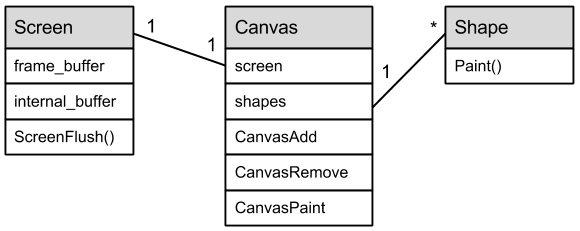
\includegraphics[width=350px]{graphics/graphics_UML.png}
  \caption{UML for the main part of graphics}
\end{figure}

\subsubsection{Images}
For all images the 24 bit version of the {\bf BMP} (Bitmap file format) was implemented. This is
done by the object {\bf Bitmap} is hidden behind the {\bf Image} object so that it is easy to add
more file formats. The reason that bitmap was chosen is that the 24 bit version of it corresponds
almost directly to the layout of the framebuffer, so the implementation was straight forward.

\subsubsection{Graphical objects}
Both objects for drawing lines and rectangles are where used only in the testing of the graphics module
and are not used in the game. They serve as examples on how to develop more graphical objects.
